\documentclass[11pt]{beamer}
\setbeamertemplate{footline}{
    \vspace{0.5cm}
}
\usetheme{metropolis}
\usefonttheme{professionalfonts}
\metroset{outer/numbering=none}
\metroset{outer/progressbar=frametitle}
\metroset{background=light}
\usepackage[math-style=TeX]{unicode-math}
\setmainfont[Ligatures=TeX]{Fira Sans}
% \setmainfont[Ligatures=TeX]{TeX Gyre Pagella}
% \setsansfont[Ligatures=TeX]{TeX Gyre Pagella}
% \setmathfont[Scale=MatchLowercase]{TeX Gyre Pagella Math}
\setmathfont[Scale=MatchLowercase,math-style=TeX]{xits-math.otf}
\usepackage{appendixnumberbeamer}
\usepackage{booktabs}
\usepackage[backend=biber,style=chem-acs,autocite=footnote]{biblatex}
\addbibresource{talk_brainowl.bib}
%% A couple of useful operators
\DeclareMathOperator*{\argmax}{arg\,max}
\DeclareMathOperator*{\argmin}{arg\,min}
%% Citations
\newrobustcmd*{\footprnifullcite}{\AtNextCite{\renewbibmacro{title}{}\renewbibmacro{in:}{}
\renewbibmacro{date}{}\renewbibmacro{note+pages}{}}\footfullcite}
\newrobustcmd*{\footlessfullcite}{\AtNextCite{\renewbibmacro{title}{}\renewbibmacro{in:}{}}\footfullcite}
%% Title / Front matter
\title{Introducing the BrainOwl}
\date{Wolberslab Lab Meeting, 30.1.2019}
\author{José Pedro Valdés Herrera}
\institute{\includegraphics[scale=0.2]{figures/DZNE_CMYK.png}\hspace{1cm}
  \includegraphics[scale=0.15]{figures/wolberslab_neg.png}}

\begin{document}

\maketitle

\section{fMRI univariate data analysis}

\begin{frame}
    \frametitle{fMRI data}

    The data resulting from fMRI is 4 dimensional (structural is 3-D). The extra
    time dimension allows us to analyse how brain activity changes during the
    task.

    \vspace*{-0.25cm}

    \begin{center}
        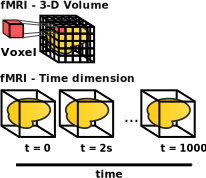
\includegraphics[scale=0.25]{figures/4d_data.png}
    \end{center}

\end{frame}
\begin{frame}
    \frametitle{Putting it all together}
    
    We can analyse the data to detect changes in activation using a General
    Linear Model (GLM), a massive-univariate analysis.

    \begin{center}
        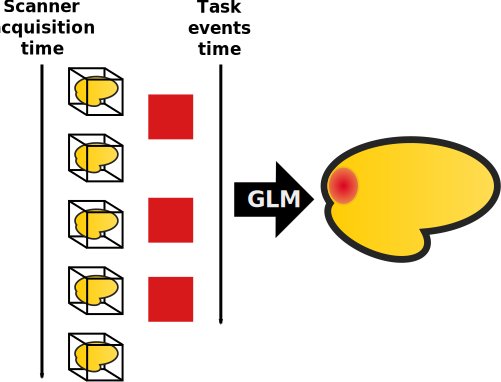
\includegraphics[scale=0.15]{figures/glm.png}
    \end{center}

\end{frame}

\section{fMRI multivariate analysis: decoding}
\label{sec:Decoding}

\begin{frame}
    \frametitle{Asking about categories}

    Maybe we would like to ask different scientific questions:
    \begin{enumerate}
        \item Can we distinguish categories from the task?
        \item Can we find cluster of voxels that discriminate among those categories?
    \end{enumerate}

    \begin{center}
        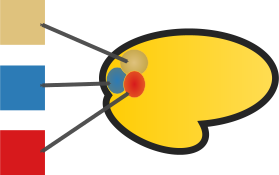
\includegraphics[scale=0.2]{figures/decoding.png}
    \end{center}

\end{frame}

\begin{frame}
    \frametitle{Model}
    Our proposal to answer those questions is to use a linear model. 

    \[y = Xw\]

    But, we have too many voxels (features) and too few images (samples). That
    is why we add an extra term to the problem to be solved called
    regularization, $J(w)$.

    \[\hat{w} = \underset{w}{\operatorname{arg\,min}} \,
        \mathcal{L}\left(y, X, w \right) + J(w) \]

    The solution that we obtain is a vector of weights, $\hat{w}$ with one
    weight per voxel: the weight map.  

\end{frame}

\begin{frame}{If things were this easy\ldots}
    Only two features (e.g., voxels) and many samples:

    \begin{center}
        \includegraphics[scale=0.3]{figures/grad_descent_result.png}        
    \end{center}

    In neuroimaging, we have thousands of features and we cannot plot the data.
    Instead, we show the weight map.

\end{frame}

\begin{frame}{A real experiment}

    In this task, participants could be in any of four different
    rooms\footlessfullcite{shine-2016}.

    \begin{columns}
        \begin{column}{0.5\textwidth}
            \begin{center}
                \includegraphics[width=0.5\textwidth]{figures/4_rooms.jpg}
            \end{center}
        \end{column}
        \begin{column}{0.5\textwidth}
            \begin{center}
                \includegraphics[width=0.5\textwidth]{figures/4_rooms_stimuli.jpg}
            \end{center}
        \end{column}
    \end{columns}
\end{frame}

\begin{frame}[squeeze]{Decoding a real experiment}

    \vspace*{-0.9cm}

    \begin{center}
        \includegraphics[scale=0.7]{figures/lsvc_l2-axial.png}
    \end{center}

    \vspace*{-0.2cm}

    \begin{enumerate}
        \item The accuracy (ACC) tells us most of the time the right room is
            identified (25\% is random guess).
        \item The weight map is \emph{dense}: all weights are $\neq$ 0.
    \end{enumerate}

    Which voxels are the most relevant?

\end{frame}
\begin{frame}
    \frametitle{Sparsity}

    We can also find a \emph{sparse} solution, i.e., many voxel weights are set
    to 0.
    
    \vspace*{-0.9cm}

    \begin{center}
        \includegraphics[scale=0.7]{figures/lsvc_l1-axial.png}
    \end{center}

    \vspace*{-0.2cm}

    \begin{enumerate}
        \item Accuracy is even better.
        \item Non-relevant voxels are set to 0, but some relevant may be too
            (e.g., correlated voxels)!
    \end{enumerate}

    Is the solution unique?

\end{frame}

\begin{frame}
  \frametitle{Is the solution unique? Not necessarily}
  An example of a highly sparse model: SVC with $l_1$ regularization and Haxby's
  faces vs. houses
    \begin{center}
      \includegraphics[scale=0.22]{figures/haxby_svc_plotmap_7e41.png}
      \includegraphics[scale=0.22]{figures/haxby_svc_plotmap_b073.png}
    \end{center}
    The outcome after running the same analysis with the same conditions: two
    different weight maps.
\end{frame}

\section{Structured sparsity}
\label{sec:Structured sparsity}

% option [t] causes text to be flushed to the top
\begin{frame}
    \frametitle{Why structured sparsity?\footprnifullcite{baldassarre2012a}}

    Summary so far:

    \begin{center}
        \begin{tabular}[h]{@{}lll@{}}
            & Pros & Cons \\
            \cmidrule(r){2-3}
            Dense ($l_2$) & stable & all voxels appear relevant \\
            Sparse ($l_1$) & few chosen voxels & unstable
        \end{tabular}
    \end{center} 
    
    \pause

    Structured sparsity offers a middle ground solution that is stable and
    selects whole relevant areas.

\end{frame}

\begin{frame}
    \frametitle{Structured sparsity}
    In a decoding analysis wishlist,
    \begin{itemize}
        \item take into consideration spatial and temporal information, \pause
        \item recover the \emph{true} weight maps, \pause
        \item ease interpretation of results. \pause
    \end{itemize}
    % \footlessfullcite{Grosenick2013} 

    To favour structured sparsity solutions, we need to use particular
    regularization terms.

\end{frame}

\begin{frame}
    \frametitle{BrainOwl}
    BrainOwl is a classifier based on the \emph{Ordered Weighted} $l_1$
    (OWL)\footlessfullcite{zeng2014-owl, bogdan-2015} norm.

    \[J_v(w) = \sum_{i=1}^{n} |w|_{[i]} v_i = v^T |w|_{\downarrow}\]

    The OWL norm is robust to correlations and can be implemented efficiently.

\end{frame}

\begin{frame}
    \frametitle{Rooms question revisited}

    \vspace*{-2cm}

    \begin{center}
        \includegraphics[scale=0.7]{figures/brainowl-axial.png}
    \end{center}

    \begin{enumerate}
        \item High accuracy ensures we can distinguish rooms.
        \item Weight map shows now only selected areas.
    \end{enumerate}

\end{frame}

\begin{frame}
    \frametitle{Summary: dense, sparse, and structured sparse}

    \begin{center}
        \includegraphics[scale=0.45]{figures/dense_sparse_structured-sparse.png}
    \end{center}
\end{frame}


\begin{frame}
    \frametitle{Final words}

    BrainOwl was developed for whole brain decoding, but it is not only limited
    to that. It can be used with any categorical data (classification) that you
    have. From other neuroimaging techniques (e.g. MEG, EEG) to behavioral
    tests, for example.

    Useful links:
    \begin{itemize}
        \item BrainOwl \\ \texttt{github.com/jpvaldes/brainowl}
            \\ Soon in \texttt{www.wolberslab.net}
            \\ Simply install with \texttt{pip install brainowl}
        \item nilearn contains alternative decoders (TV-L$_1$, GraphNet) \\ 
            \texttt{nilearn.github.io}
        \item scikit-learn, ML library \\ \texttt{scikit-learn.org}
    \end{itemize}
\end{frame}

\begin{frame}[standout]
    Thank you! \\
    Now, \emph{live demo time}.
\end{frame}

%% -- backup slides --
%% backup slides go after appendix as normal frames. See theme documentation
%% and include \usepackage{appendixnumberbeamer} so that they do not count
%% towards the total number of slides in the main presentation
\appendix
\section{Extra slides}
\begin{frame}[t]
    \frametitle{Other structured sparsity decoders}
    
    \vspace*{-1cm} 

    \begin{center}
        \includegraphics[scale=0.35]{figures/template_and_weights_4_clfs.png}
    \end{center}

    There are other structured sparsity classifiers implemented like
    \emph{Sparse Total Variation} (TV-$l_1$)\footprnifullcite{gramfort2013} or
    \emph{Graph-Net}\footlessfullcite{grosenick2013}.

\end{frame}
\begin{frame}[t,shrink]
  \frametitle{Structured Sparsity: Graph-Net\footlessfullcite{grosenick2013}}
  Basic idea: look for a regularization term promoting sparsity and imposing
  structure at the same time.

  The starting point is the \emph{Elastic-Net}, a regression problem with
  \[J(\mathbf{w}) = \lambda_{1}\lVert{\mathbf{w}}\rVert_{1} + 
    \lambda_{2}\lVert{\mathbf{w}}\rVert_{2}^{2}\]

  where the \(l_{2}\) term is substituted by a new term
  \(\lambda_{G}\lVert{\mathbf{w}}\rVert_{G}^{2}\). The new term can incorporate
  spatial and temporal information, e.g. using the discrete Laplacian.

  Derivatives of the coefficients encourage smooth solutions
  (i.e., penalize roughness) while the $l_{1}$ term promotes sparse solutions. 

\end{frame}
\begin{frame}
  \frametitle{Structured Sparsity: TV-$l_1$\footprnifullcite{gramfort2013}}
  The idea behind \emph{Sparse Total Variation} (TV-$l_{1}$) is similar to
  Graph-Net. 

  \[J(\mathbf{w}) = \lambda \left( \lVert{\mathbf{w}}\rVert _{1} + 
   \lVert{\nabla\mathbf{w}}\rVert _{1}\right) \]

  This time, the TV term, $\lVert{\nabla\mathbf{w}}\rVert _{1}$ favors sharp
  contours and piece-wise constant solutions to the regression problem, in contrast
  with the Graph-Net that prefers smoother solutions.
\end{frame}
\begin{frame}[t]
  \frametitle{Example: Noisy Data}
  A set of simulated noisy data consisting of 30 samples and 2 clases. 
  \begin{center}
    \includegraphics[scale=0.25]{figures/weights_synthetic_data_2.62_cbc.png} 
  \end{center}
\end{frame}
\begin{frame}[t]
  \frametitle{Example: Noisier Data}
  Same ground truth but noisier data.
  \begin{center}
    \includegraphics[scale=0.25]{figures/weights_sparse_synthetic_data_1.39_cbc.png} 
  \end{center}
\end{frame}
\begin{frame}
  \frametitle{Regularization: Purpose}
  Regularization
  \begin{itemize}
  \item helps with overfitting,
  \item can do feature selection ($\rightarrow$ sparsity),
  \item and is necessary to solve the mathematical problem when the number of
    dimensions is very high (because it is ill-posed).
  \end{itemize}

\end{frame}
\begin{frame}
  \frametitle{Regularization: How does it do it?}
  Regularization is a term, \(J(\mathbf{w})\), added to the optimization problem:
  % \[\mathbf{y} = \mathbf{Xw} + \lambda{}J(\mathbf{w})\]
  \[\hat{\mathbf{w}} = \argmin_{\mathbf{w}} \lVert \mathbf{y} - \mathbf{Xw}
    \rVert^{2}_{2} + \lambda{}J(\mathbf{w})\]
  \begin{center}
    \begin{tabular}[h]{@{}lll@{}}
      & \(J(\mathbf{w})\) & Effect \\
      \cmidrule(r){2-3}
      Ridge, \(l_{2}\) & \(\lVert{\mathbf{w}}\rVert{}^{2}_{2} = \sum_{i=1}^{N}w_{i}^{2}\) & Shrinkage \\
      Lasso, \(l_{1}\) & \(\lVert{\mathbf{w}}\rVert_{1} = \sum_{i=1}^{N}\left| w_{i} \right|\) & Sparsity \\
    \end{tabular}
  \end{center}
  \begin{center}
    \includegraphics[scale=0.25]{figures/l1_l2_geometry.png}
  \end{center}
\end{frame}
\begin{frame}
  \frametitle{Regularization: Effect on Coefficients}
  \begin{columns}
    \begin{column}{0.5\linewidth}
      \includegraphics[scale=0.2]{figures/houses_grid.png}
    \end{column}
    \begin{column}{0.5\linewidth}
      \vspace{-0.6cm}
      \begin{center}
        \includegraphics[scale=0.2]{figures/logistic_regression_l2_coef_path.png}
      \end{center}
      \begin{center}
        \includegraphics[scale=0.2]{figures/logistic_regression_l1_coef_path.png}
      \end{center}
    \end{column}
  \end{columns}
\end{frame}

\end{document}
% Local Variables:
% TeX-engine: xetex
% coding: utf-8
% mode: latex
% TeX-master: t
% TeX-command-extra-options: "-shell-escape"
% End:
